\documentclass[11pt,letterpaper]{article}
\usepackage{iftex}
\ifXeTeX
  \usepackage{fontspec}   % Tectonic / XeLaTeX
\else
  \usepackage[utf8]{inputenc}   % pdfLaTeX (Overleaf)
  \usepackage[T1]{fontenc}
\fi
\IfFileExists{spanish.ldf}{\usepackage[spanish,es-noshorthands,es-tabla]{babel}}{%
  \renewcommand{\contentsname}{Índice}\renewcommand{\figurename}{Figura}\renewcommand{\tablename}{Cuadro}}
\usepackage{lmodern}
\usepackage[margin=2.3cm,headheight=34pt,headsep=14pt,includehead]{geometry}
\usepackage{amsmath,amssymb}
\usepackage{graphicx}
\usepackage{booktabs}
\usepackage{array}
\usepackage{float}
\usepackage{xcolor}
\usepackage{listings}
\usepackage{fancyhdr}
\usepackage{caption}
\usepackage{enumitem}
\usepackage{url}
\usepackage[hidelinks]{hyperref}

% GENERADO por ref/analisis.py: numeros que se citan en el texto. No editar a mano.
\newcommand{\GeoPrac}{0,961}
\newcommand{\GeoPracCyM}{0,959}
\newcommand{\GanaPrac}{5}
\newcommand{\NPrac}{10}
\newcommand{\PeorPrac}{6.837}
\newcommand{\GeoPracInv}{1,042}
\newcommand{\GeoPracInvCyM}{1,042}
\newcommand{\GanaPracInv}{4}
\newcommand{\NPracInv}{10}
\newcommand{\PeorPracInv}{7.535}
\newcommand{\GeoAli}{0,971}
\newcommand{\GeoAliCyM}{0,972}
\newcommand{\GanaAli}{15}
\newcommand{\NAli}{70}
\newcommand{\PeorAli}{5.924}
\newcommand{\GeoAliInv}{1,030}
\newcommand{\GeoAliInvCyM}{1,029}
\newcommand{\GanaAliInv}{16}
\newcommand{\NAliInv}{70}
\newcommand{\PeorAliInv}{6.782}
\newcommand{\WPrac}{6.636}
\newcommand{\CyMPrac}{6.497}
\newcommand{\OrdenesPrac}{2}
\newcommand{\ExpoPrac}{100}
\newcommand{\WPracInv}{15.280}
\newcommand{\CyMPracInv}{15.348}
\newcommand{\OrdenesPracInv}{2}
\newcommand{\ExpoPracInv}{100}
\newcommand{\TbW}{9.995}
\newcommand{\TbOrdenes}{1}
\newcommand{\TbPerdida}{5}
\newcommand{\TbCyM}{6.695}
\newcommand{\TbPeor}{12}
\newcommand{\TbAprobados}{4/4}
\newcommand{\TecCincoRazon}{1,002}
\newcommand{\TecCincoExpo}{100}
\newcommand{\TecCincoGeo}{0,932}
\newcommand{\TecHoraRazon}{1,028}
\newcommand{\TecHoraExpo}{99}
\newcommand{\TecHoraGeo}{1,540}
\newcommand{\TecRondasRazon}{1,004}
\newcommand{\TecRondasExpo}{100}
\newcommand{\TecRondasGeo}{1,085}
\newcommand{\TecSubeRazon}{1,007}
\newcommand{\TecSubeExpo}{100}
\newcommand{\TecSubeGeo}{1,462}
\newcommand{\TecBajaRazon}{1,002}
\newcommand{\TecBajaExpo}{99}
\newcommand{\TecBajaGeo}{0,748}
\newcommand{\PracMin}{72}
\newcommand{\PracMax}{190}
\newcommand{\PracIni}{151}
\newcommand{\PracFin}{98}
\newcommand{\PracVR}{0,53}
\newcommand{\PracAC}{-0,11}
\newcommand{\CiclosPromSw}{406,6}
\newcommand{\CiclosPeorSw}{443}
\newcommand{\ICPromSw}{180,1}
\newcommand{\CPISw}{2,26}
\newcommand{\PalabrasSw}{159}
\newcommand{\TickCeroSw}{1.458}
\newcommand{\MopsSw}{1,32}
\newcommand{\MIPSSw}{11,07}
\newcommand{\PctRtresSw}{19,6}
\newcommand{\SpeedupSw}{1,00}
\newcommand{\CiclosPromShift}{382,6}
\newcommand{\CiclosPeorShift}{419}
\newcommand{\ICPromShift}{168,1}
\newcommand{\CPIShift}{2,28}
\newcommand{\PalabrasShift}{118}
\newcommand{\TickCeroShift}{1.376}
\newcommand{\MopsShift}{1,40}
\newcommand{\MIPSShift}{10,98}
\newcommand{\PctRtresShift}{18,5}
\newcommand{\SpeedupShift}{1,06}
\newcommand{\CiclosPromMul}{133,4}
\newcommand{\CiclosPeorMul}{139}
\newcommand{\ICPromMul}{57,6}
\newcommand{\CPIMul}{2,32}
\newcommand{\PalabrasMul}{121}
\newcommand{\TickCeroMul}{1.213}
\newcommand{\MopsMul}{4,02}
\newcommand{\MIPSMul}{10,80}
\newcommand{\PctRtresMul}{6,1}
\newcommand{\SpeedupMul}{3,05}
\newcommand{\CiclosPromMulShift}{109,4}
\newcommand{\CiclosPeorMulShift}{115}
\newcommand{\ICPromMulShift}{45,6}
\newcommand{\CPIMulShift}{2,40}
\newcommand{\PalabrasMulShift}{80}
\newcommand{\TickCeroMulShift}{1.131}
\newcommand{\MopsMulShift}{4,91}
\newcommand{\MIPSMulShift}{10,42}
\newcommand{\PctRtresMulShift}{5,1}
\newcommand{\SpeedupMulShift}{3,72}
\newcommand{\NTicks}{320.000}
\newcommand{\OpsTick}{21,5}
\newcommand{\BytesTick}{12}
\newcommand{\IntensidadOp}{1,79}
\newcommand{\Presupuesto}{2.262}
\newcommand{\MulPorTick}{4,5}
\newcommand{\FracMul}{72,0}
\newcommand{\FracDup}{8,4}
\newcommand{\CiclosMulSw}{65}
\newcommand{\AmdahlFShift}{8,4}
\newcommand{\AmdahlSShift}{3,4}
\newcommand{\AmdahlPredShift}{1,06}
\newcommand{\AmdahlMedShift}{1,06}
\newcommand{\AmdahlMaxShift}{1,09}
\newcommand{\AmdahlFMul}{72,0}
\newcommand{\AmdahlSMul}{6,5}
\newcommand{\AmdahlPredMul}{2,56}
\newcommand{\AmdahlMedMul}{3,05}
\newcommand{\AmdahlMaxMul}{3,57}
\newcommand{\AmdahlFMulShift}{80,3}
\newcommand{\AmdahlSMulShift}{6,0}
\newcommand{\AmdahlPredMulShift}{3,02}
\newcommand{\AmdahlMedMulShift}{3,72}
\newcommand{\AmdahlMaxMulShift}{5,09}
\newcommand{\LCOriginal}{1191}
\newcommand{\LCPctOriginal}{93,0}
\newcommand{\FmaxOriginal}{42,5--45,5}
\newcommand{\LCSw}{985}
\newcommand{\LCPctSw}{77,0}
\newcommand{\FmaxSw}{45,7--46,6}
\newcommand{\LCShift}{1253}
\newcommand{\LCPctShift}{97,9}
\newcommand{\FmaxShift}{41,3--43,3}
\newcommand{\LCMul}{1185}
\newcommand{\LCPctMul}{92,6}
\newcommand{\FmaxMul}{46,7--47,4}
\newcommand{\LCMulShift}{1444}
\newcommand{\LCPctMulShift}{112,8}
\newcommand{\AhorroRAM}{206}
\newcommand{\LCLibres}{295}
\newcommand{\CostoMul}{200}
\newcommand{\CostoShift}{268}
\newcommand{\ExtGeo}{2,005}
\newcommand{\ExtMediana}{2,391}
\newcommand{\ExtPcinco}{1,068}
\newcommand{\ExtPeor}{0,970}
\newcommand{\ExtPierde}{0,7}
\newcommand{\ExtGanaCym}{100}
\newcommand{\ExtDDmed}{3.465}
\newcommand{\ExtDDpnoventa}{9.117}
\newcommand{\ExtExpo}{51}
\newcommand{\ExtCortaGeo}{1,070}
\newcommand{\ExtCortaMediana}{1,000}
\newcommand{\ExtCortaPcinco}{0,979}
\newcommand{\ExtCortaPeor}{0,899}
\newcommand{\ExtCortaPierde}{9,2}
\newcommand{\ExtCortaGanaCym}{65}
\newcommand{\ExtCortaDDmed}{0}
\newcommand{\ExtCortaDDpnoventa}{2.144}
\newcommand{\ExtCortaExpo}{26}
\newcommand{\TendGeo}{1,111}
\newcommand{\TendMediana}{1,170}
\newcommand{\TendPcinco}{0,476}
\newcommand{\TendPeor}{0,400}
\newcommand{\TendPierde}{41,0}
\newcommand{\TendGanaCym}{34}
\newcommand{\TendDDmed}{6.404}
\newcommand{\TendDDpnoventa}{11.156}
\newcommand{\TendExpo}{100}
\newcommand{\TendCortaGeo}{1,015}
\newcommand{\TendCortaMediana}{1,012}
\newcommand{\TendCortaPcinco}{0,747}
\newcommand{\TendCortaPeor}{0,468}
\newcommand{\TendCortaPierde}{47,7}
\newcommand{\TendCortaGanaCym}{25}
\newcommand{\TendCortaDDmed}{1.862}
\newcommand{\TendCortaDDpnoventa}{4.233}
\newcommand{\TendCortaExpo}{100}
\newcommand{\CymGeo}{1,115}
\newcommand{\CymMediana}{1,158}
\newcommand{\CymPcinco}{0,478}
\newcommand{\CymPeor}{0,399}
\newcommand{\CymPierde}{42,2}
\newcommand{\CymCortaGeo}{1,016}
\newcommand{\CymCortaMediana}{1,012}
\newcommand{\CymCortaPcinco}{0,744}
\newcommand{\CymCortaPeor}{0,461}
\newcommand{\CymCortaPierde}{47,7}
\newcommand{\NVentanas}{2.732}
\newcommand{\ExtGeoDosmilveintidos}{1,784}
\newcommand{\ExtPierdeDosmilveintidos}{1,4}
\newcommand{\TendPierdeDosmilveintidos}{61}
\newcommand{\ExtGeoDosmilveintitres}{2,139}
\newcommand{\ExtPierdeDosmilveintitres}{0,4}
\newcommand{\TendPierdeDosmilveintitres}{30}
\newcommand{\ExtGeoDosmilveinticuatro}{2,143}
\newcommand{\ExtPierdeDosmilveinticuatro}{0,0}
\newcommand{\TendPierdeDosmilveinticuatro}{30}
\newcommand{\MCN}{1.000}
\newcommand{\MCPeor}{0,861}
\newcommand{\MetaW}{23.215}
\newcommand{\MetaWTend}{11.060}
\newcommand{\MetaCym}{9.695}
\newcommand{\MetaWCorta}{9.920}
\newcommand{\MetaWTendCorta}{11.375}
\newcommand{\MetaCymCorta}{11.375}
\newcommand{\MetaTickMax}{10.965}
\newcommand{\MetaTickMin}{17.084}
\newcommand{\ExtPalabras}{63}
\newcommand{\ExtCiclosProm}{12,2}
\newcommand{\ExtCiclosPeor}{22}
\newcommand{\ExtIC}{5,5}
\newcommand{\ExtICPeor}{10}
\newcommand{\ExtCPI}{2,24}
\newcommand{\ExtMops}{5,19}
\newcommand{\ExtMIPS}{11,16}
\newcommand{\ExtOpsTick}{2,5}
\newcommand{\ExtBytesTick}{8}
\newcommand{\ExtNTicks}{1.039.948}
\newcommand{\ExtPctRtres}{1,0}
\newcommand{\ExtSpeedupMul}{11}
\newcommand{\ExtSpeedupSw}{33}
\newcommand{\TbExtW}{9.995}
\newcommand{\TbExtOrdenes}{1}
\newcommand{\TbExtPerdida}{5}
\newcommand{\TbExtCyM}{6.695}
\newcommand{\TbExtPeor}{12}
\newcommand{\TbExtAprobados}{4/4}
\newcommand{\TbMetaW}{23.215}
\newcommand{\TbMetaOrdenes}{8}
\newcommand{\TbMetaPerdida}{3.296}
\newcommand{\TbMetaCyM}{9.695}
\newcommand{\TbMetaPeor}{12}
\newcommand{\TbMetaAprobados}{4/4}
\newcommand{\RefW}{23.215}
\newcommand{\RefOrdenes}{8}
\newcommand{\RefComisiones}{40}
\newcommand{\RefPerdida}{3.296}
\newcommand{\RefCymPerdida}{9.300}
\newcommand{\ExtTiempoProm}{0,49}
\newcommand{\ExtTiempoPeor}{0,88}
\newcommand{\ExtTickCero}{16}
\newcommand{\AEntra}{3}
\newcommand{\ASale}{1}
\newcommand{\CSube}{0}
\newcommand{\CBaja}{24}
\newcommand{\BExceso}{12}


\graphicspath{{figuras/}}
\captionsetup{font=small,labelfont=bf}
\setlist{nosep}
\setlist[itemize]{topsep=3pt,itemsep=3pt}
\renewcommand{\lstlistingname}{Código}
\newcommand{\fuente}[1]{\par\vspace{3pt}{\centering\footnotesize\emph{Fuente: #1}\par}}
\newcommand{\FechaEntrega}{27 de noviembre de 2026}

\lstdefinelanguage{rvasm}{
  morekeywords={li,lw,sw,lbu,sb,add,addi,sub,andi,ori,beq,bne,beqz,bnez,bltu,bgeu,blt,bge,bgez,bltz,
    j,jal,jalr,ret,mv,mul8,slli},
  sensitive=false, morecomment=[l]{\#}}
\lstset{language=rvasm, basicstyle=\ttfamily\footnotesize, commentstyle=\color{gray},
  keywordstyle=\color{blue!60!black}\bfseries, columns=fullflexible, frame=single,
  framerule=0.4pt, rulecolor=\color{black}, xleftmargin=2pt, xrightmargin=2pt,
  captionpos=b, aboveskip=8pt, belowskip=6pt}

\pagestyle{fancy}
\fancyhf{}
\fancyhead[L]{
\includegraphics[height=1.15cm]{logo_header.png}}
\fancyhead[C]{Arquitectura de Computadores}
\fancyfoot[L]{\footnotesize Facultad Ingeniería y Ciencias Aplicadas\\ Universidad de los Andes}
\fancyfoot[R]{\thepage}
\renewcommand{\headrulewidth}{0.4pt}
\renewcommand{\footrulewidth}{0.4pt}

\begin{document}

%=============================================================================
% Portada
%=============================================================================
\begin{titlepage}
\thispagestyle{empty}
\centering
\vspace*{0.5cm}

\includegraphics[height=4.6cm]{logo_portada.png}\par
\vspace{0.9cm}
{\large UNIVERSIDAD DE LOS ANDES\par}
{Facultad de Ingeniería y Ciencias Aplicadas\par}
{Arquitectura de Computadores 2026-2\par}
\vspace{1.5cm}
{\LARGE\bfseries Entrega N°4\par}
\vspace{0.5cm}
{\large Pochoco Trader: co-diseño hardware/software sobre Espino Core\par}
\vspace{1.5cm}
{Grupo 2:\par}
Josefa Alcaíno Lira\par
Felipe Izcúe Ferrer\par
Martín Norton Haigis\par
\vspace{1.0cm}
Profesor de Cátedra: Jorge Gómez M.\par
Ayudantes:\par
Chen Shi Ye\par
Nicolás Villegas\par
\vspace{0.6cm}
{\FechaEntrega\par}
\vfill
\end{titlepage}

%=============================================================================
% Resumen e índice
%=============================================================================
\begin{center}\textbf{Resumen}\end{center}
\vspace{2pt}
En este informe se documenta un agente de inversión que corre en el Pochoco SoC, con el procesador
Espino RV32E, sobre la Go Board. En cada tick la FPGA maestra entrega por SPI el precio de una acción
y el programa responde si compra, vende o mantiene, y en qué cantidad. Las series de la competencia son
ventanas de 20.000 minutos de acciones reales llevadas a $[100, 255]$: el mínimo vale 100 y el máximo
255, y los dos aparecen siempre. La serie de práctica se reconstruyó exacta desde precios de Meta. El
agente, llamado \emph{extremos} y entregado en su versión D, compra cuando el precio vale 100 (o 122
si el 100 y el 255 ya pasaron) y vende cuando vale 255 (o 225 si el máximo ya pasó); antes del primer
extremo compra 15 acciones si el precio sube 29 sobre el inicial. En la serie de práctica termina con
\$\MetaW{} contra \$\MetaCym{} de comprar y mantener. En \NVentanas{} ventanas posibles de Meta, Apple,
Netflix, AMD y Tesla multiplica la plata por \ExtGeo{} en media geométrica, contra \CymGeo{} de comprar
y mantener, y pierde en el \ExtPierde\,\% de ellas. Los parámetros (225, 122 y 29) se ajustaron con esas
mismas ventanas, así que este resultado es dentro de muestra; un Montecarlo con series sintéticas, que no se
usaron para elegirlos, lo revisa en la sección 3. El programa en assembly tiene \ExtPalabras{}
palabras, no multiplica ni desplaza, y toma \ExtCiclosProm{} ciclos por tick en promedio y
\ExtCiclosPeor{} en el peor caso, el \ExtPctRtres\,\% del tiempo disponible en la ronda más rápida.
Decide lo mismo que la referencia en Python, salvo en los dos primeros ticks, que llegan durante el reset, aprueba el testbench del curso y se probó en la placa. El
estudio de co-diseño, hecho con el algoritmo anterior, mostró que una instrucción propia \texttt{mul8}
acelera el tick \SpeedupMul{} veces con \CostoMul{} celdas más, mientras que un barrel shifter acelera
\SpeedupShift{} veces y las dos juntas no caben en la iCE40 HX1K; el encapsulado de la Go Board no tiene PLL.
Con el algoritmo final no hacen falta \texttt{mul8} ni shifter: la variante entregada es el Espino sin
instrucciones nuevas, con una sola mejora de hardware, el registro NUEVO del esclavo SPI y la lectura
bloqueante, con \LCSw{} celdas lógicas y una frecuencia máxima de \FmaxSw\,MHz.

\newpage
\tableofcontents
\newpage

%=============================================================================
\section{Introducción}

El Proyecto 4 consiste en diseñar un agente de inversión que corra en el Pochoco SoC \cite{pochoco},
que integra el procesador Espino con el conjunto de instrucciones RV32E de RISC-V \cite{riscv}, sobre
la Go Board. Una FPGA maestra, operada por el curso, transmite por SPI el precio de una acción tick a
tick. En cada tick el programa del grupo decide si compra, vende o mantiene, y en qué cantidad. Además
de ganar plata en la competencia, el enunciado \cite{enunciado} pide decidir qué parte del algoritmo
va en software y qué parte en hardware, y justificarlo con las métricas vistas en clases: ciclos, CPI,
Ops/s, celdas lógicas y frecuencia máxima.

El protocolo es el siguiente. La maestra comparte SCLK, MOSI y CS\_n con todos los grupos, y cada grupo
tiene su propia línea MISO. En cada período $T$ baja CS\_n, manda el precio $p_n$ como un byte entre 1 y
255 y lee el byte que el grupo dejó en el registro DECISION. Ese byte es la respuesta al precio anterior,
$p_{n-1}$, y la maestra lo ejecuta al precio $p_n$. Si el programa no alcanza a escribir una decisión
nueva, la maestra repite la anterior. El byte de decisión tiene la acción en los bits 7 y 6
(\texttt{00} mantener, \texttt{01} comprar, \texttt{10} vender) y la cantidad $q \le 63$ en los bits 5 a 0.

El trabajo se organiza según las actividades del enunciado \cite{enunciado}:

\begin{itemize}
\item Sección 2: entorno y reproducibilidad.
\item Sección 3: algoritmo de predicción y decisión (3.1).
\item Sección 4: implementación en assembly (3.2).
\item Sección 5: co-diseño hardware/software (3.3).
\item Sección 6: prueba en la placa y competencia en vivo (3.4).
\end{itemize}

El Cuadro~\ref{tab:params} resume los parámetros de la competencia. El testbench del curso descuenta
9,5\,$\mu$s de la transacción SPI, así que a 25\,MHz la ronda 3 deja \Presupuesto{} ciclos para decidir.
Una entrega se considera correcta cuando el programa decide lo mismo que su referencia, el testbench del
curso aprueba y el diseño cabe y cierra timing en la FPGA.

\begin{table}[H]
\centering\small
\caption{Parámetros de la competencia.}
\label{tab:params}
\begin{tabular}{lrrr}
\toprule
Ronda & Período $T$ & Ciclos a 25\,MHz & Ciclos para decidir \\
\midrule
1 & 10\,ms & 250.000 & 249.762 \\
2 & 1\,ms & 25.000 & 24.762 \\
3 & 0,1\,ms & 2.500 & \Presupuesto \\
\midrule
\multicolumn{4}{l}{Caja inicial \$10.000 y 0 acciones; comisión fija \$5 por orden ejecutada;}\\
\multicolumn{4}{l}{sin ventas en corto ni deuda; precios enteros entre 1 y 255; $q \le 63$; SCLK $\le$ 1\,MHz.}\\
\bottomrule
\end{tabular}
\fuente{Enunciado del Proyecto 4 \cite{enunciado}. Caja y comisión son valores referenciales.}
\end{table}

\textbf{Repositorio.} El código, los testbenches, los resultados y el README con las instrucciones
completas están en \url{https://github.com/F-Izcue-223/Proyecto-4-Arquitectura-de-Computadores}
\cite{repo}.

%=============================================================================
\section{Entorno y reproducibilidad}

Los resultados se generaron en computadores con Windows 11 y Git Bash, con la OSS CAD Suite para
la síntesis y la simulación. El Cuadro~\ref{tab:versiones} resume las versiones de las herramientas,
registradas también en el README.

\begin{table}[H]
\centering\small
\caption{Versiones de las herramientas.}
\label{tab:versiones}
\begin{tabular}{ll}
\toprule
Componente & Versión \\
\midrule
OSS CAD Suite & build 2026-08-24 \\
Yosys & 0.68+120 (git sha1 a34d3baae) \\
nextpnr-ice40 & 0.11.1-9-gb17408e2 \\
Icarus Verilog & 14.0 (devel) s20260301 \\
icestorm (icepack, iceprog) & los de la misma OSS CAD Suite \\
Python & 3.11.15 (numpy 1.26.4, matplotlib 3.8.0, pandas 2.1.4) \\
GNU Make & 4.4.1 \\
Sistema & Windows 11 + Git Bash \\
\bottomrule
\end{tabular}
\fuente{Elaboración propia, desde el README del repositorio.}
\end{table}

\textbf{Estructura del repositorio.} \texttt{rtl/} contiene el SoC y el Espino Core, con las variantes
de hardware detrás de \texttt{ifdef}; \texttt{sw/} el programa \texttt{trade.s} y su imagen de memoria;
\texttt{tools/} el assembler \texttt{pochoasm.py}, el programador de la placa y el simulador; \texttt{ref/}
la referencia en Python y los análisis; \texttt{sim/} y \texttt{tb/} los testbenches propios y el del curso;
\texttt{data/series/} las series de práctica; \texttt{resultados/} los CSV de cada medición; y
\texttt{informe/} y \texttt{docs/} este informe y las guías.

\textbf{Historia del repositorio.} El primer commit del repositorio base es \texttt{pochoco\_soc} sin
cambios. El segundo trae los cambios del grupo en el Proyecto 2: el reset de encendido de 4095 ciclos
y el contador de ciclos. Con \texttt{git diff} contra esos commits se ve todo lo que se hizo en este
proyecto.

\textbf{Cómo reproducir.} El diseño de la competencia es el que sale sin ninguna opción de compilación,
con la versión D de \texttt{trade.s}. Desde la raíz del repositorio:

\begin{lstlisting}[language={},caption={Ensamblar \texttt{trade.s} y correr el testbench del curso.}]
python3 tools/pochoasm.py sw/trade.s -o sw/trade.hex      # make hex
make tb                                                    # Testbenchs aprobados: 4/4
make tb-meta                                               # practica_meta completa (lento)
make bin && make prog                                      # sintesis y grabado en la Go Board
python3 ref/analisis.py                                    # regenera tablas y figuras del informe
\end{lstlisting}

El programa se ensambla con \texttt{tools/pochoasm.py}, el assembler del grupo del Proyecto 2, porque
en estos computadores no hay toolchain de RISC-V. Las tablas, las figuras y los números que se citan en
el texto los genera \texttt{ref/analisis.py} desde los archivos de \texttt{resultados/}, de modo que
ningún número del informe se copió a mano.

\textbf{Versión entregada.} Las constantes de \texttt{trade.s} que definen la versión D se muestran en el
Cuadro~\ref{tab:constantes}. Las demás versiones (A a G) salen del mismo archivo cambiando constantes al
ensamblar (\texttt{-D}), con \texttt{tools/versiones.py}.

\begin{table}[H]
\centering\small
\caption{Constantes de \texttt{trade.s} en la versión D, la entregada.}
\label{tab:constantes}
\begin{tabular}{llp{7.5cm}}
\toprule
Constante & Valor & Significado \\
\midrule
\texttt{MINIMO}, \texttt{MAXIMO} & 100, 255 & extremos de la normalización \\
\texttt{TOMA\_GANANCIA} & 225 & techo después de que apareció el 255 \\
\texttt{RECOMPRA} & 122 & piso después de que aparecieron los dos extremos \\
\texttt{ANCLA} & 29 & subida sobre el primer precio que dispara la compra parcial \\
\texttt{ANCLA\_ORDEN} & \texttt{0x4F} & comprar 15 acciones \\
\texttt{COMPRAR}, \texttt{VENDER} & \texttt{0x7F}, \texttt{0xBF} & comprar 63 y vender 63 \\
\bottomrule
\end{tabular}
\fuente{Elaboración propia, desde \texttt{sw/trade.s}.}
\end{table}

%=============================================================================
\section{Algoritmo de predicción y decisión}

\subsection{Cómo se arman las series de la competencia}

El 17 de noviembre el curso publicó una serie de práctica nueva, \texttt{tb/practica\_meta.csv}, con
el formato de la competencia: 20.000 precios de Meta entre febrero y mayo de 2022, uno por minuto de
mercado, normalizados entre 100 y 255. En la competencia se usarán períodos no informados de Meta,
Apple, Netflix, AMD o Tesla entre 2022 y 2024, normalizados igual. Que las series de la competencia
vayan entre 100 y 255 es entonces una suposición basada en el formato de esta serie de práctica: el
enunciado \cite{enunciado} solo indica precios enteros entre 1 y 255, y el agente depende de esa
suposición (ver la sección de límites).

Se bajaron las barras de 1 minuto de esas cinco acciones entre 2022 y 2024 (datos de Alpaca
publicados en Hugging Face). Con el cierre de Meta en horario regular (9:30 a 16:00 de Nueva York) se
buscó la ventana de 20.000 minutos que más se parece a la práctica. La ventana que parte el 23 de
febrero de 2022 a las 15:20, llevada linealmente a $[100, 255]$ y redondeada, da la serie de práctica
exacta: los 20.000 precios son iguales. La normalización es
\begin{equation}
p_n = \operatorname{round}\!\left(100 + 155\,\frac{x_n - \min x}{\max x - \min x}\right),
\end{equation}
con el mínimo y el máximo tomados sobre toda la ventana.

Con eso se puede armar cualquier serie que podría tocar en la competencia. Cada empresa tiene unas
273.000 ventanas posibles. Para evaluar se tomó una cada 500 minutos: \NVentanas{} ventanas en total
(\texttt{ref/minuto.py} y \texttt{ref/competencia.py}).

\subsection{Lo que implica la normalización}

La normalización usa el mínimo y el máximo de toda la ventana, que incluye el futuro. Eso deja
información sobre el futuro en el nivel del precio. La Figura~\ref{fig:nivel} muestra el retorno
promedio desde un tick hasta el final de la ventana, según el nivel del precio en ese tick. Bajo 170
el precio tiende a subir y sobre 180 tiende a bajar.

\begin{figure}[H]
\centering
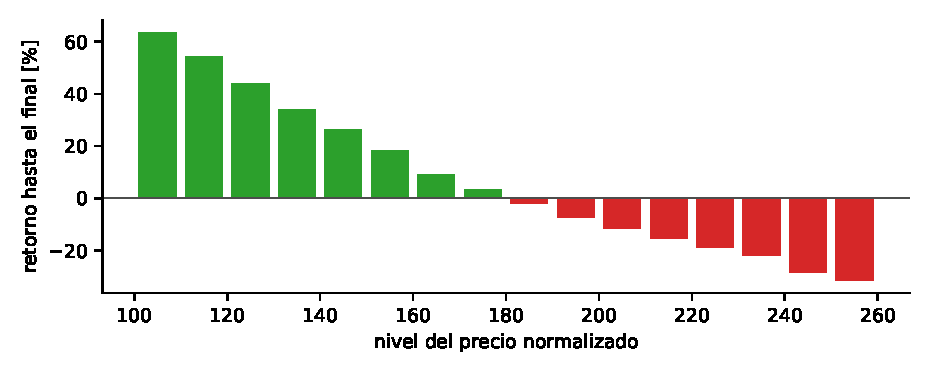
\includegraphics[width=0.85\textwidth]{nivel_retorno.pdf}
\caption{Retorno hasta el final de la ventana según el nivel del precio, en las \NVentanas{} ventanas
(media geométrica por tramo de 10). Fuente: elaboración propia.}
\label{fig:nivel}
\end{figure}

Hay dos hechos más fuertes, que valen en todas las ventanas.
\begin{enumerate}
\item El precio nunca baja de 100 ni sube de 255.
\item El 100 y el 255 aparecen alguna vez dentro de la ventana.
\end{enumerate}
Si el precio vale 100 y todavía no apareció el 255, el 255 tiene que venir después. Comprar en ese
momento y vender en el 255 multiplica la plata por 2,55, menos comisiones. Si el 255 ya pasó, comprar
en 100 no puede perder, porque el precio ya no baja de 100.

\subsection{La regla}

El algoritmo final se llama \emph{extremos}. Recuerda qué extremos ya aparecieron y decide con
comparaciones contra un piso y un techo (Cuadro~\ref{tab:reglas}).

\begin{table}[H]
\centering\small
\caption{Reglas del algoritmo final (versión D). El piso vale 100 hasta que aparecieron el 100 y el 255,
y desde ahí vale 122. El techo vale 255 hasta que aparece el 255, y desde ahí vale 225.}
\label{tab:reglas}
\begin{tabular}{lll}
\toprule
Precio & Decisión & Por qué \\
\midrule
$p \le$ piso & dentro (comprar 63) & 100 es el mínimo; 122 recompra cerca del piso \\
$p \ge$ techo & fuera (vender 63) & 255 es el máximo; 225 toma la ganancia \\
$p \ge p_0 + 29$, sin extremos & comprar 15, después mantener & subidas del comienzo (ancla) \\
$p \le p_0$, sin extremos & fuera (vender 63) & la subida no siguió \\
entre medio & no cambia & \\
\bottomrule
\end{tabular}
\fuente{Elaboración propia.}
\end{table}

El agente parte fuera, con piso 100 y techo 255. Cuando aparece el 255 el techo baja a 225, porque
desde ahí no hay garantía de que el precio vuelva a 255. Cuando ya aparecieron el 100 y el 255 no queda
ninguna garantía, pero comprar cerca del piso arriesga poco, porque el precio no baja de 100: el piso
sube a 122.

El 100 y el 255 salen del formato de la serie de práctica y no de ajustar datos; se supone que las series de la competencia lo tienen igual. El 225, el 122 y el
ancla de 29 sí se ajustaron: un optimizador exploró 82.976 combinaciones de reglas y parámetros y
solo conservó las que cumplían los límites de riesgo, todas de la familia del ancla; la mejor contra
rivales con reglas parecidas fue la versión D (sección~\ref{sec:versiones}). Cualquier valor de
recompra entre 115 y 140 da casi lo mismo, así que el valor exacto importa poco.

La razón del techo en 225 y no más alto es la competencia. Se compite contra otros grupos con reglas
parecidas, y entre reglas casi iguales la mayoría de las rondas termina en empate, así que decide el
resultado cara a cara. Un techo menor al máximo gana en más rondas de las que pierde contra un rival
que use 100/255 puro.

Las prácticas con la maestra mostraron que si la serie parte subiendo, la regla simple no compra nada
hasta ver el 100, porque antes del primer extremo no hay ninguna garantía. Para no perder esas subidas
se agregó un \emph{ancla}: mientras no aparece ni el 100 ni el 255, si el precio sube 29 sobre el primero
($p_0$) se compran 15 acciones una sola vez, y si vuelve a $p_0$ se vende todo. Comprando todo, el ancla
ganaba cara a cara a la regla sin ancla, pero una serie que sube y baja varias veces sin tocar los
extremos la hacía perder hasta 21\,\% en una ronda. Con solo 15 acciones el daño queda acotado: en
13.652 ventanas reales de 22 acciones la peor ronda de la versión D es $-4{,}8$\,\%, la probabilidad de
perder es 0,6\,\% y le gana cara a cara a la versión con ancla 30 (+12,2\,\% neto). Esos números salen
del optimizador del grupo (\texttt{docs/ruta-optimizacion.md}, sección 19).

\subsection{Cómo se decide la cantidad $q$}

Si está dentro, el programa manda comprar 63. Si está fuera, manda vender 63. No lleva la cuenta de
la caja ni de las acciones.

Esto funciona por cómo ejecuta la maestra, según la tarea \texttt{ejecutar} del testbench. Una
compra se recorta a lo que alcanza con la caja. Una venta se recorta a las acciones que hay. Una
orden que queda en 0 no se ejecuta y no paga comisión. Cerca de 100, \$10.000 alcanzan para unas 99
acciones: la posición se llena en dos ticks (63 y el resto) y después la misma orden ya no hace nada.
El ancla es la excepción: compra solo 15 acciones, a propósito, para acotar la pérdida.

También resuelve el deadline. Si el programa no alcanza a responder, la maestra repite la orden
anterior, que es la misma que se quería mandar. No se arriesga la ruina \cite{naval}, porque no hay
deuda ni ventas en corto y la maestra nunca ejecuta más de lo que alcanza.

\subsection{Implementable con los recursos de la FPGA}

El enunciado pide que el algoritmo use solo lo que existe en la FPGA. \emph{Extremos} usa aritmética
entera de 8 bits sobre los precios y solo comparaciones sin signo: no hay multiplicaciones, divisiones
ni desplazamientos, que el Espino no tiene. No guarda series de precios, y como no lleva contabilidad
tampoco necesita memoria de datos: el programa ocupa \ExtPalabras{} palabras de instrucciones y 0 de
datos. Su estado son siete registros (piso, techo, decisión vigente y la bandera de que ya apareció el
100, más el ancla). Por eso corre en el Espino sin instrucciones nuevas y sin memoria extra, y el SoC
completo ocupa \LCSw{} de las 1280 celdas lógicas de la iCE40 HX1K.

\subsection{Comparación con las referencias}

Se comparó el agente con las dos referencias del enunciado, no operar y comprar y mantener, en la serie de
práctica completa (Cuadro~\ref{tab:referencias}). Las reglas de ejecución son las de la maestra, la
comisión paga \$5 por orden y la pérdida máxima es la caída desde un peak de patrimonio, como la mide
el testbench.

\begin{table}[H]
\centering\small
\caption{Agente contra las dos referencias en \texttt{practica\_meta.csv} (20.000 ticks).}
\label{tab:referencias}
\begin{tabular}{lrrrr}
\toprule
Estrategia & Patrimonio final [\$] & Órdenes & Comisiones [\$] & Pérdida máxima [\$] \\
\midrule
Agente (versión D) & 23.215 & 8 & 40 & 3.296 \\
No operar & 10.000 & 0 & 0 & 0 \\
Comprar y mantener & 9.695 & 1 & 5 & 9.300 \\
\bottomrule
\end{tabular}

\fuente{Elaboración propia con \texttt{ref/mercado.py}, que reproduce las reglas del testbench.}
\end{table}

El agente termina con \$\RefW{} en \RefOrdenes{} órdenes y \$\RefComisiones{} de comisiones, contra
\$\MetaCym{} de comprar y mantener. La serie sube hasta 190, cae hasta 72 y termina en 98: comprar y mantener
queda con una caída de \$\RefCymPerdida{} desde su peak y el agente con \$\RefPerdida. La
Figura~\ref{fig:meta} muestra la serie. El 255 aparece en el tick \MetaTickMax{} y el 100 en el tick
\MetaTickMin, después del máximo. El agente compra cerca de 100 y vende en 225. El algoritmo anterior,
\emph{tendencia}, termina con \$\MetaWTend.

\begin{figure}[H]
\centering
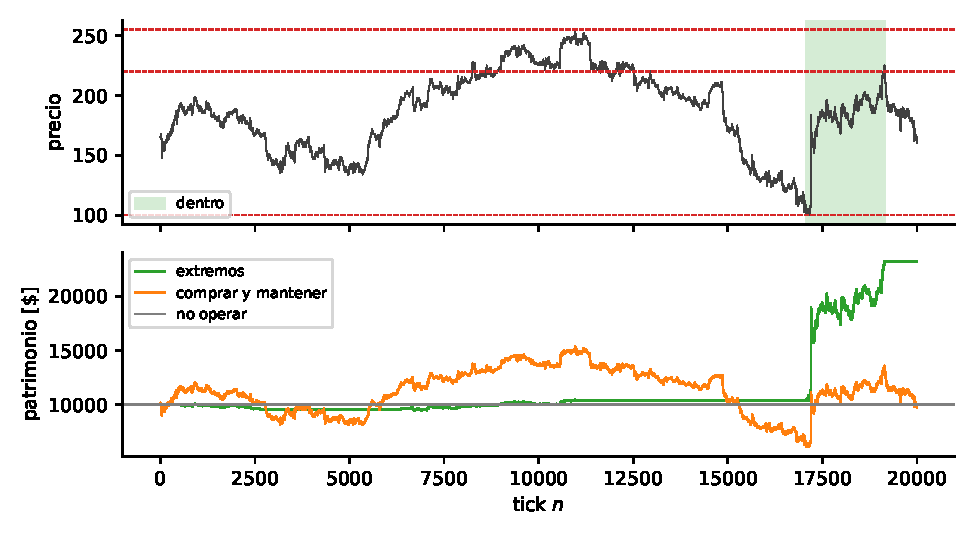
\includegraphics[width=0.9\textwidth]{practica_meta.pdf}
\caption{Serie de práctica \texttt{practica\_meta.csv}. Arriba, el precio, los niveles 100, 225 y 255
y en verde los ticks dentro. Abajo, el patrimonio. Fuente: elaboración propia.}
\label{fig:meta}
\end{figure}

\subsection{Ganancia y riesgo en ventanas reales}

Se supone que cada ronda de la competencia usa una serie de 20.000 ticks, como la práctica. Como el
testbench corre por defecto solo los primeros 2000, se evaluaron los dos casos en las \NVentanas{} ventanas, con las reglas de
la maestra y contra comprar y mantener calculado como en el testbench.

\begin{table}[H]
\centering\small
\caption{Patrimonio final dividido por \$10.000 en las \NVentanas{} ventanas. Geo.\ es la media
geométrica. Pierde es la fracción de ventanas que terminan bajo \$10.000. La pérdida máxima es la
caída desde un peak, en pesos, como la mide el testbench.}
\label{tab:competencia}
\footnotesize\setlength{\tabcolsep}{3.5pt}
\begin{tabular}{llrrrrrrr}
\toprule
Ronda & Algoritmo & Geo. & Mediana & 5\,\% peor & Peor & Pierde & Gana a CyM & Pérd. máx. p95 [\$] \\
\midrule
20\,000 ticks & extremos (final) & 2,005 & 2,391 & 1,068 & 0,970 & 0,7\,\% & 100\,\% & 9.117 \\
 & tendencia (anterior) & 1,111 & 1,170 & 0,476 & 0,400 & 41,0\,\% & 34\,\% & 11.156 \\
 & comprar y mantener & 1,115 & 1,158 & 0,478 & 0,399 & 42,2\,\% & -- & -- \\
\midrule
2000 ticks & extremos (final) & 1,070 & 1,000 & 0,979 & 0,899 & 9,2\,\% & 65\,\% & 2.144 \\
 & tendencia (anterior) & 1,015 & 1,012 & 0,747 & 0,468 & 47,7\,\% & 25\,\% & 4.233 \\
 & comprar y mantener & 1,016 & 1,012 & 0,744 & 0,461 & 47,7\,\% & -- & -- \\
\bottomrule
\end{tabular}

\fuente{Elaboración propia con \texttt{ref/competencia.py}.}
\end{table}

Con la serie completa el agente multiplica la plata por \ExtGeo{} en media geométrica, contra
\CymGeo{} de comprar y mantener. Termina con pérdida en el \ExtPierde\,\% de las ventanas, contra el
\CymPierde\,\% de comprar y mantener, y su peor ventana deja \ExtPeor{} veces la plata inicial. Ese es
el riesgo de mercado que queda: comprar en 100 cuando el máximo ya pasó y que la ventana termine cerca
de 100. Está con acciones el \ExtExpo\,\% del tiempo.

\begin{figure}[H]
\centering
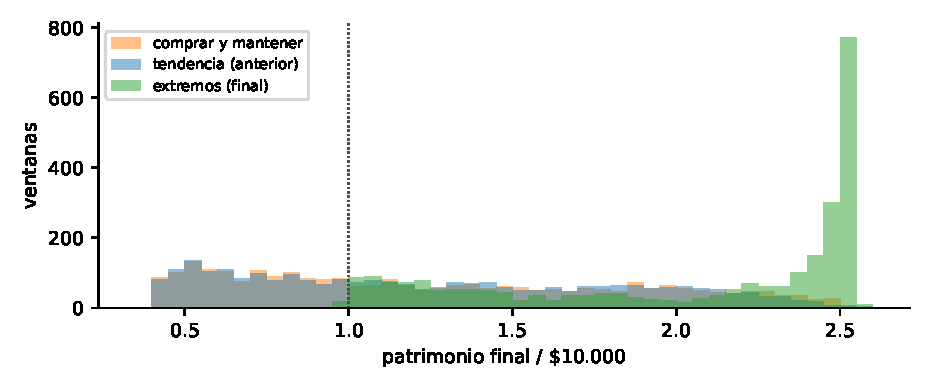
\includegraphics[width=0.85\textwidth]{competencia_hist.pdf}
\caption{Patrimonio final en las \NVentanas{} ventanas, ronda de 20.000 ticks. Fuente: elaboración propia.}
\label{fig:hist_comp}
\end{figure}

El resultado es parejo entre empresas y entre años (Cuadro~\ref{tab:grupos}). En 2022, el año de
caída de las tecnológicas, el algoritmo anterior perdía en el \TendPierdeDosmilveintidos\,\% de las
ventanas y el final en el \ExtPierdeDosmilveintidos\,\%.

\begin{table}[H]
\centering\small
\caption{Media geométrica del patrimonio final por empresa y por año de inicio de la ventana.}
\label{tab:grupos}
\begin{tabular}{lrrrrrrrr}
\toprule
Ronda de 20\,000 ticks & META & AAPL & NFLX & AMD & TSLA & 2022 & 2023 & 2024 \\
\midrule
extremos (final) & 2,137 & 2,009 & 2,120 & 1,933 & 1,842 & 1,784 & 2,139 & 2,143 \\
tendencia (anterior) & 1,244 & 1,113 & 1,270 & 1,014 & 0,950 & 0,867 & 1,309 & 1,236 \\
comprar y mantener & 1,234 & 1,121 & 1,285 & 1,019 & 0,951 & 0,866 & 1,326 & 1,234 \\
\bottomrule
\end{tabular}

\fuente{Elaboración propia con \texttt{ref/competencia.py}.}
\end{table}

Con rondas de 2000 ticks la ventaja es menor. En la mayoría de las ventanas el 100 no aparece en los
primeros 2000 ticks y el agente no opera: la mediana es \$10.000 y solo está con acciones el
\ExtCortaExpo\,\% del tiempo. Aun así termina con pérdida en el \ExtCortaPierde\,\% de las ventanas
(contra \CymCortaPierde\,\% de comprar y mantener), su peor ventana deja \ExtCortaPeor{} veces la plata
y su media geométrica es \ExtCortaGeo, contra \CymCortaGeo. Le gana a comprar y mantener en el
\ExtCortaGanaCym\,\% de las ventanas. En la práctica con 2000 ticks termina con \$\MetaWCorta{} y
comprar y mantener con \$\MetaCymCorta.

\subsection{Montecarlo: otras series con la misma normalización}

Las ventanas reales son de solo cinco acciones y tres años. Para ver si el resultado depende de ellas
se generaron \MCN{} series sintéticas de 20.000 minutos por escenario, con comportamientos distintos,
y se normalizaron igual que la práctica (\texttt{ref/montecarlo.py}). El último escenario arma cada
serie con días reales de las cinco acciones puestos en orden al azar.

\begin{table}[H]
\centering\small
\caption{Montecarlo: patrimonio final dividido por \$10.000 de la versión D en \MCN{} series por
escenario. ``Solo 100/255'' es la media geométrica de la regla sin toma de ganancia ni recompra.}
\label{tab:montecarlo}
\begin{tabular}{lrrrrrrr}
\toprule
Escenario & Geo. & 5\,\% peor & Peor & Pierde & Órdenes & Solo 100/255 & CyM \\
\midrule
paseo aleatorio & 1,883 & 1,068 & 0,990 & 0,6\,\% & 4,7 & 1,833 & 0,990 \\
tendencia al alza (+40\,\%) & 2,509 & 2,410 & 1,409 & 0,0\,\% & 4,2 & 2,512 & 2,131 \\
tendencia a la baja ($-$30\,\%) & 1,102 & 0,999 & 0,976 & 12,3\,\% & 2,3 & 1,097 & 0,464 \\
volatilidad triple & 1,857 & 1,055 & 0,944 & 1,0\,\% & 4,7 & 1,809 & 0,995 \\
vuelve a la media & 2,095 & 1,190 & 0,895 & 0,7\,\% & 7,0 & 1,980 & 0,987 \\
momentum & 1,905 & 1,065 & 0,978 & 0,8\,\% & 4,6 & 1,864 & 1,010 \\
saltos de $\pm$3\,\% & 1,873 & 1,055 & 0,861 & 1,0\,\% & 4,5 & 1,826 & 0,980 \\
días reales al azar & 1,865 & 1,036 & 0,901 & 1,6\,\% & 4,4 & 1,828 & 1,002 \\
\bottomrule
\end{tabular}

\fuente{Elaboración propia con \texttt{ref/montecarlo.py}.}
\end{table}

En todos los escenarios el agente termina sobre comprar y mantener, salvo en el de tendencia al
alza, donde este último gana más. Su peor serie deja \MCPeor{} veces la plata inicial. El único escenario
con pérdidas frecuentes (12,3\,\%) es la tendencia a la baja: ahí el mínimo suele estar al final, el
agente compra en 100 cerca del cierre y pierde las comisiones y el redondeo, a lo más 2,4\,\%. Comprar
y mantener pierde más de la mitad en ese mismo escenario. La toma de ganancia y la recompra mejoran a la regla simple en siete de los ocho
escenarios, también en series que no se usaron para elegirlas; en la tendencia al alza dan lo mismo.

\subsection{Versiones probadas y elección de la versión D}
\label{sec:versiones}

El algoritmo cambió dos veces antes de llegar a \emph{extremos}.
\begin{itemize}
\item La primera versión invertía más cuando el precio estaba bajo en el rango de 1 a 255. La primera
serie de práctica no recorría ese rango y se descartó.
\item La segunda, \emph{tendencia}, usaba dos medias móviles de 64 y 512 ticks y tres banderas con
histéresis. Se validó con 15 acciones tecnológicas reales y estaba dentro casi todo el tiempo. En las
ventanas de la competencia queda igual que comprar y mantener (\TendGeo) y pierde en el
\TendPierde\,\% de ellas. Con ella se hizo el estudio de co-diseño de la sección~\ref{sec:codiseno}.
\end{itemize}

Sobre \emph{extremos} se probaron variantes que salen del mismo programa cambiando constantes
(Cuadro~\ref{tab:versiones_alg}). En la serie de práctica del curso y en las otras siete prácticas que
recibió el grupo, la versión D le ganó a los rivales con reglas parecidas en las ocho
(\texttt{docs/ruta-optimizacion.md}, sección 27), y la F y la G, que compran todo al inicio si el primer
precio es alto, no mejoraron de forma pareja. Probadas las versiones G, F y D con la maestra del curso el
25 de noviembre, la D fue la que mejor se comportó y es la que quedó grabada en la placa.

\begin{table}[H]
\centering\small
\caption{Versiones de \emph{extremos} probadas.}
\label{tab:versiones_alg}
\begin{tabular}{lp{11cm}}
\toprule
Versión & Diferencia con la regla base \\
\midrule
A & ancla 30, recompra 120 (la versión de la primera entrega del algoritmo) \\
B & sin ancla: la más segura, peor ronda $-3$\,\% \\
C & ancla 26, recompra 117 \\
\textbf{D} & \textbf{ancla 29, recompra 122: la entregada} \\
E & la D, pero con ancla solo si el primer precio es al menos 160 \\
F & si el primer precio es al menos 170 compra todo al inicio y espera el 255; si no, la D \\
G & sin ancla; compra todo si el primer precio es al menos 180 o si llega a 240, y espera el 255 \\
\bottomrule
\end{tabular}
\fuente{Elaboración propia, desde \texttt{tools/versiones.py}.}
\end{table}

Sobre la regla final se probaron además otros umbrales de compra y venta (110 y 250, 120 y 240, etc.),
entrar por partes, un modo distinto para rondas cortas y medias móviles encima de la regla. Ninguna mejoró
de forma pareja.

\subsection{Límites}

La regla depende de que la serie de la competencia esté normalizada como la práctica. Si el mínimo no
llegara a 100, el agente no operaría y terminaría con \$10.000: no pierde, pero tampoco gana. Se supone que
la normalización es la misma que la de la práctica; el enunciado no lo garantiza. Otro grupo puede
llegar a la misma regla; en ese caso la diferencia la hacen la toma de ganancia en 225, la recompra en
122 y el ancla.

%=============================================================================
\section{Implementación en assembly}

\subsection{Ciclo principal}

El programa está en \texttt{sw/trade.s} y tiene \ExtPalabras{} palabras. No multiplica ni desplaza,
así que no necesita instrucciones nuevas. Tiene dos fases. En la fase 1, que dura hasta que aparece el
primer extremo, vigila el ancla. En la fase 2 cada tick espera el precio, lo compara con el piso y el
techo y escribe DECISION (Código~\ref{cod:fase2}).

\begin{lstlisting}[caption={Un tick de la fase 2 de \texttt{trade.s}.},label={cod:fase2}]
espera:
    lw   a1, 12(s0)             # NUEVO (bloqueante): t1 + precio
decidir:
    bgeu a2, a1, piso           # p <= piso vigente
    bgeu a1, a4, techo          # p >= techo vigente
    sw   a5, 8(s0)              # DECISION (no cambia)
    sw   a1, 0(sp)              # displays: precio en hexadecimal
    j    espera
piso:
    sw   a0, 8(s0)              # DECISION = comprar, antes que nada
    mv   a5, a0
    sw   a1, 0(sp)
    bltu gp, a1, espera         # p > 100: recompra, no es el minimo
    li   s1, 1                  # aparecio el 100
    beq  a4, a3, espera         # el 255 todavia no aparece
    addi a2, t1, RECOMPRA       # ya aparecieron los dos
    j    espera
techo:
    sw   ra, 8(s0)              # DECISION = vender, antes que nada
    mv   a5, ra
    sw   a1, 0(sp)
    bltu a1, a3, espera         # p < 255: toma de ganancia
    addi a4, t1, TOMA_GANANCIA  # aparecio el 255
    beqz s1, espera             # el 100 todavia no aparece
    addi a2, t1, RECOMPRA       # ya aparecieron los dos
    j    espera
\end{lstlisting}

El programa espera el precio con una sola instrucción: lee el registro NUEVO del esclavo SPI, que
entrega el aviso de precio nuevo en el bit 31 y el precio en los bits 7 a 0, y la lectura no termina
hasta que llega un precio (sección~\ref{sec:velocidad}). Como el precio llega con el bit 31 en 1, el
piso y el techo se guardan sumados a \texttt{0x8000\_0000} y se comparan sin signo (\texttt{bgeu},
\texttt{bltu}). El caso común, en que el precio no toca el piso ni el techo, pasa por las dos comparaciones
sin saltar y escribe DECISION de inmediato. Cuando la decisión cambia, se escribe DECISION antes de
actualizar el piso y el techo. El Espino no tiene \texttt{ble}: la comparación $p \le \text{piso}$ se
escribe como \texttt{bgeu a2, a1}, que es $\text{piso} \ge p$.

La fase 1 (Código~\ref{cod:fase1}) guarda $p_0$ y $p_0 + 29$ (a lo más 255, para que ``$p \ge$ ancla arriba''
cubra también ``$p \ge 255$'') y compara cada precio con los dos. Si sube al ancla compra 15 acciones una
sola vez y desde el tick siguiente manda mantener; si vuelve a $p_0$ vende todo. Cuando aparece el 100 o el
255 salta a la fase 2.

\begin{lstlisting}[caption={Fase 1 de \texttt{trade.s}: el ancla.},label={cod:fase1}]
espera_ancla:
    lw   a1, 12(s0)             # NUEVO (bloqueante)
    bgeu a1, t2, ancla_alto     # p >= p0 + ANCLA (o p >= 255)
    bgeu tp, a1, ancla_bajo     # p <= p0 (o p <= 100)
    sw   a5, 8(s0)              # DECISION (no cambia)
    sw   a1, 0(sp)
    j    espera_ancla
ancla_alto:
    bgeu a1, a4, techo          # p >= 255: pasa a la fase 2
    beqz a5, ancla_tengo        # ya compro la parte: sigue "mantener"
    sw   t0, 8(s0)              # DECISION = comprar 15, una sola vez
    li   a5, 0                  # desde el tick siguiente: mantener
    sw   a1, 0(sp)
    j    espera_ancla
\end{lstlisting}

\subsection{Registros, memoria y operaciones que el Espino no tiene}

El Cuadro~\ref{tab:registros} resume el uso de registros y memoria. Los precios son enteros de 8 bits y
todas las constantes también, así que no se necesita punto fijo. El Espino no tiene multiplicación ni
división y tiene los desplazamientos deshabilitados; \emph{extremos} no los necesita, porque solo compara.
El algoritmo anterior sí multiplicaba, y ahí la multiplicación se resolvió con sumas y desplazamientos por
software o con la instrucción \texttt{mul8} (sección~\ref{sec:codiseno}). Como el Espino tampoco tiene
\texttt{ble}, las comparaciones $\le$ se escriben con los operandos al revés.

\begin{table}[H]
\centering\small
\caption{Uso de registros y memoria en \texttt{trade.s}.}
\label{tab:registros}
\begin{tabular}{lll}
\toprule
Registro & Contenido & Vida \\
\midrule
\texttt{s0} & base SPI \texttt{0x8001\_0000} & todo el programa \\
\texttt{sp} & base de periféricos \texttt{0x8000\_0000} & todo el programa \\
\texttt{t1} & \texttt{0x8000\_0000}, base de las constantes & todo el programa \\
\texttt{gp}, \texttt{a3} & 100 y 255, el mínimo y el máximo (+ \texttt{t1}) & todo el programa \\
\texttt{a2} & piso vigente: 100 y después 122 (+ \texttt{t1}) & todo el programa \\
\texttt{a4} & techo vigente: 255 y después 225 (+ \texttt{t1}) & todo el programa \\
\texttt{s1} & 1 si ya apareció el 100 & todo el programa \\
\texttt{a0}, \texttt{ra} & \texttt{0x7F} y \texttt{0xBF}, para escribir DECISION sin un \texttt{li} & todo el programa \\
\texttt{tp}, \texttt{t2}, \texttt{t0} & ancla: $p_0$, $p_0+29$ (a lo más 255) y la orden ``comprar 15'' & hasta el primer extremo \\
\texttt{a5} & decisión vigente (\texttt{0x7F} o \texttt{0xBF}) & todo el programa \\
\texttt{a1} & precio $p$ (+ \texttt{t1}) & un tick \\
\midrule
RAM \texttt{0x000}--\texttt{0x0FB} & programa (\ExtPalabras{} palabras); no usa la RAM de datos & \\
\bottomrule
\end{tabular}
\fuente{Elaboración propia, desde \texttt{sw/trade.s}.}
\end{table}

\subsection{Mismas decisiones que la referencia}

Se comprobó de tres formas que \texttt{trade.s} toma las mismas decisiones que \texttt{ref/trader.py}.

La primera es un simulador de instrucciones del Espino escrito en Python (\texttt{ref/espino\_iss.py}).
Corre el \texttt{.hex} de la versión D sobre la práctica, 35 ventanas de la competencia y las 16 series del
estudio anterior, \ExtNTicks{} ticks en total. En todos los ticks el byte escrito fue el mismo que el de
Python.

La segunda es el RTL completo en Icarus Verilog con el testbench del curso y la serie de práctica
completa de 20.000 ticks, con el período de la ronda 3. Se comparó, tick a tick, el byte que ejecutó la maestra
con el de Python: coinciden en 19.998 de los 20.000 ticks, incluida la entrada del ancla en el tick 536 (comprar
15). Los dos primeros ticks difieren porque sus precios llegan mientras el SoC sigue en su reset de encendido, y la
orden que Python habría dado (vender sin tener acciones) no se ejecuta. La versión anterior del ancla (30 en vez de
29) sí difiere en el tick 536, así que la prueba distingue ambas.

La tercera es el testbench del curso con su serie por defecto, que aprueba \TbExtAprobados{}: patrimonio
\$\TbExtW{} con \TbExtOrdenes{} orden y peor caso precio $\to$ decisión de \TbExtPeor{} ciclos de
\Presupuesto{} disponibles. Con la práctica nueva completa el patrimonio final es \$\TbMetaW{} con
\TbMetaOrdenes{} órdenes, y comprar y mantener da \$\TbMetaCyM{} (\texttt{make tb-meta}, una copia del
testbench con otra serie y otro largo). El testbench manda los dos primeros precios mientras el SoC sigue
en su reset de encendido, que dura 164\,$\mu$s; con esta regla eso no cambia nada.

\subsection{Mediciones por tick}

El IC y los ciclos de un tick se miden desde que el programa lee el precio hasta que llega de nuevo a la
espera del precio siguiente, es decir, el tick completo.
El Cuadro~\ref{tab:extremos} resume las mediciones sobre \ExtNTicks{} ticks, en el caso promedio y en el
peor caso, y las compara con el tiempo disponible de cada ronda. Ojo con dos ``peor caso'' distintos: el
de este cuadro (\ExtCiclosPeor{} ciclos) es la duración de un tick completo, mientras que los
\TbExtPeor{} ciclos de la subsección anterior miden solo desde que llega el precio hasta que se escribe
DECISION.

\begin{table}[H]
\centering\small
\caption{Mediciones por tick de \texttt{trade.s} a 25\,MHz. El peor caso es el tick más largo (aparece
un extremo y cambian el piso o el techo); IC y ciclos máximos pueden ocurrir en ticks distintos.}
\label{tab:extremos}
\begin{tabular}{lrr}
\toprule
Métrica & Promedio & Peor caso \\
\midrule
Instrucciones ejecutadas (IC) & 5,5 & 10 \\
Ciclos & 12,2 & 22 \\
CPI & 2,24 & -- \\
Tiempo de ejecución a 25\,MHz [$\mu$s] & 0,49 & 0,88 \\
\% de $T-T_\text{SPI}$, ronda 1 & 0,00 & 0,01 \\
\% de $T-T_\text{SPI}$, ronda 2 & 0,05 & 0,09 \\
\% de $T-T_\text{SPI}$, ronda 3 & 0,54 & 0,97 \\
\bottomrule
\end{tabular}

\fuente{Elaboración propia con \texttt{ref/verificar.py} y \texttt{ref/analisis.py}.}
\end{table}

Un tick toma \ExtIC{} instrucciones y \ExtCiclosProm{} ciclos en promedio, con CPI \ExtCPI. El peor
tick toma \ExtCiclosPeor{} ciclos. Eso es el \ExtPctRtres\,\% del tiempo disponible en la ronda 3, la
más exigente, así que las tres rondas se cumplen con mucho margen. El arranque, hasta leer el primer
precio, toma \ExtTickCero{} ciclos.

El CPI está cerca de 2,2 porque el banco de registros del Espino es una BRAM de lectura sincrónica.
Cada instrucción espera un ciclo a sus operandos. Los loads y los saltos tomados cuestan un ciclo más.

%=============================================================================
\section{Co-diseño hardware/software}
\label{sec:codiseno}

El estudio de co-diseño se hizo con el algoritmo anterior, \emph{tendencia}
(\texttt{sw/trade\_tendencia.s}), antes de conocer el formato de la competencia. Ese kernel sí
multiplicaba: llevaba dos medias móviles como sumas en buffers circulares de 64 y 512 precios y
comparaba umbrales en 64avos, con 3 a 5 multiplicaciones por tick. Un solo archivo servía para las
cuatro variantes de hardware, con las partes que cambian entre \texttt{.if HW\_MUL} y
\texttt{.if HW\_SHIFT}. Se verificó igual que el final: el mismo byte que su referencia en Python en
todos los ticks, en el simulador de instrucciones y en el RTL. Se reproduce con \texttt{ALGO=tendencia}.
Al final de la sección se revisa qué cambia con el algoritmo final.

\begin{table}[H]
\centering\small
\caption{Algoritmo anterior: IC, ciclos, CPI y tiempo por tick a 25\,MHz, y peor tick como porcentaje
del tiempo disponible ($T$ menos la transacción SPI). $^\dagger$ No cabe en la FPGA.}
\label{tab:medidas}
\begin{tabular}{lrrrrrrrrr}
\toprule
 & \multicolumn{2}{c}{IC} & \multicolumn{2}{c}{Ciclos} & & \multicolumn{2}{c}{Tiempo [$\mu$s]} & \multicolumn{2}{c}{\% de $T-T_\text{SPI}$} \\
\cmidrule(lr){2-3}\cmidrule(lr){4-5}\cmidrule(lr){7-8}\cmidrule(lr){9-10}
Variante & prom. & peor & prom. & peor & CPI & prom. & peor & R2 & R3 \\
\midrule
solo software & 180,1 & 196 & 406,6 & 443 & 2,26 & 16,3 & 17,7 & 1,8 & 19,6 \\
shifter & 168,1 & 184 & 382,6 & 419 & 2,28 & 15,3 & 16,8 & 1,7 & 18,5 \\
mul8 & 57,6 & 59 & 133,4 & 139 & 2,32 & 5,3 & 5,6 & 0,6 & 6,1 \\
mul8 + shifter$^\dagger$ & 45,6 & 47 & 109,4 & 115 & 2,40 & 4,4 & 4,6 & 0,5 & 5,1 \\
\bottomrule
\end{tabular}

\fuente{Elaboración propia con \texttt{ref/verificar.py}.}
\end{table}

\begin{figure}[H]
\centering
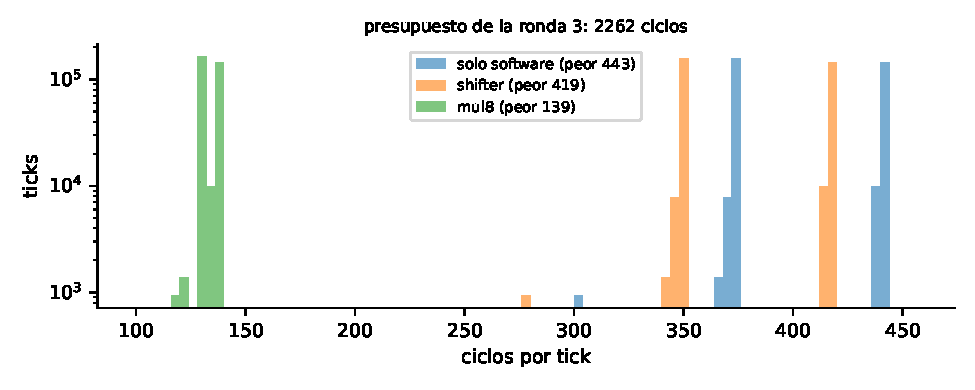
\includegraphics[width=0.85\textwidth]{ciclos_por_tick.pdf}
\caption{Algoritmo anterior: ciclos por tick en las 16 series, por variante. Fuente: elaboración propia.}
\label{fig:hist}
\end{figure}

\subsection{Dónde se van los ciclos}

El simulador de instrucciones cuenta los ciclos de cada instrucción. Con eso se armó un perfil por
parte del programa. En la versión solo software la multiplicación se lleva el \FracMul\,\% de los
ciclos. Son \MulPorTick{} multiplicaciones por tick en promedio y cada una cuesta unos \CiclosMulSw{}
ciclos. Las duplicaciones (multiplicar por 64 y por 512) son el \FracDup\,\%.

\begin{figure}[H]
\centering
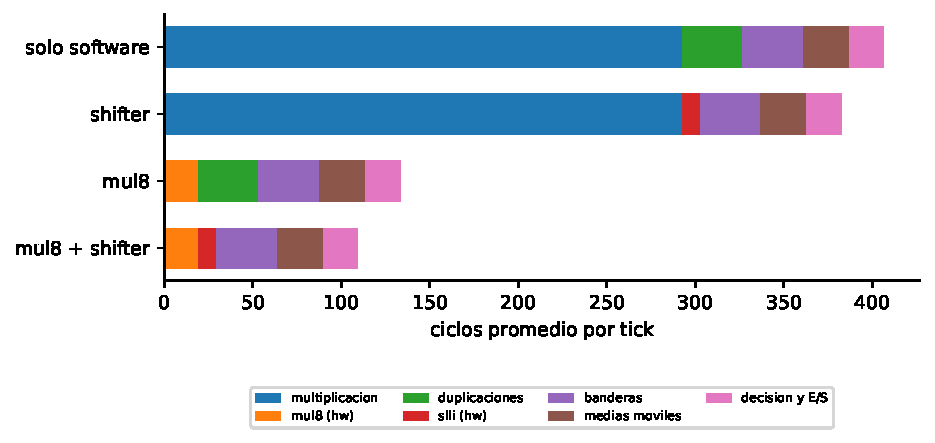
\includegraphics[width=0.85\textwidth]{perfil.pdf}
\caption{Perfil de ciclos por parte del programa en cada variante. Fuente: elaboración propia.}
\label{fig:perfil}
\end{figure}

Según la ley de Amdahl \cite{hp}, si una fracción $f$ del tiempo se acelera $s$ veces, el speedup total es
\begin{equation}
S = \frac{1}{(1-f) + f/s}.
\end{equation}
Aunque la multiplicación costara cero ciclos, el speedup no pasaría de $1/(1-f) = \AmdahlMaxMul$.
Las duplicaciones solas no darían más de \AmdahlMaxShift.

El $s$ de cada alternativa se predijo antes de construirla. Para el shifter, cada cadena de $k$ sumas
($2k$ ciclos) pasa a ser un \texttt{slli} de 2 ciclos. Para \texttt{mul8}, cada llamada a la rutina
pasa a ser una instrucción de 10 ciclos, su peor caso con un multiplicador de 8 bits.

\begin{table}[H]
\centering\small
\caption{Speedup predicho por Amdahl contra el medido. $^\dagger$ No cabe en la FPGA.}
\label{tab:amdahl}
\begin{tabular}{lrrrrr}
\toprule
Variante & $f$ & $s$ predicho & $S$ Amdahl & $S$ medido & $S_\text{máx}=1/(1-f)$ \\
\midrule
shifter & 8,4\,\% & 3,40 & 1,06 & 1,06 & 1,09 \\
mul8 & 72,0\,\% & 6,53 & 2,56 & 3,05 & 3,57 \\
mul8 + shifter$^\dagger$ & 80,3\,\% & 5,96 & 3,02 & 3,72 & 5,09 \\
\bottomrule
\end{tabular}

\fuente{Elaboración propia con \texttt{ref/verificar.py}.}
\end{table}

El speedup medido de \texttt{mul8} queda sobre el predicho. La predicción usó siempre 10 ciclos. Los
umbrales del algoritmo son números chicos y el multiplicador real termina en 3 a 5 ciclos. Para el
shifter la predicción es exacta, porque cada \texttt{slli} cuesta siempre 2 ciclos.

\subsection{Primero, liberar área}

El SoC del Proyecto 2 ocupaba \LCOriginal{} de las 1280 celdas lógicas (\LCPctOriginal\,\%). Con eso
no cabía casi nada más. Revisando la síntesis por módulo se vio que la RAM unificada usaba 93 LUTs y
117 flip-flops además de sus BRAM.

Esa lógica la agrega Yosys para emular qué devuelve una lectura de la misma dirección que se escribe
en ese ciclo. En este SoC eso no pasa. El programa no se modifica a sí mismo, y el core nunca lee y
escribe un dato en el mismo ciclo. Con el atributo \texttt{(* no\_rw\_check *)} en la memoria el SoC
bajó a \LCSw{} celdas (\LCPctSw\,\%), \AhorroRAM{} celdas menos que el SoC del Proyecto 2, sin cambiar su
comportamiento. Midiendo el diseño final con y sin el atributo, solo el atributo explica unas 200 de esas celdas
(1187 sin él y 986 con él en una corrida de nextpnr; el Cuadro de síntesis da 985 porque es el mejor de tres semillas); el resto sale de otros cambios del SoC. En una versión anterior del diseño
había dado 174 celdas. Todas las variantes parten de esta base.

\subsection{Alternativa 1: barrel shifter}

La primera alternativa fue habilitar los shifts del RV32E, que el Espino tiene deshabilitados para
ahorrar LUTs. Se implementó un solo barrel shifter a la derecha de 33 bits. El bit extra copia el signo
para SRA. Para SLL se invierte el orden de los bits a la entrada y a la salida. Así hay un shifter y
no tres.

Costó \CostoShift{} celdas y dejó la FPGA al \LCPctShift\,\%. La frecuencia máxima bajó a
\FmaxShift\,MHz porque el shifter queda en la ruta crítica de la ALU. El tick promedio bajó de
\CiclosPromSw{} a \CiclosPromShift{} ciclos, un speedup de \SpeedupShift. Es poco porque las
duplicaciones son una parte chica del perfil.

\subsection{Alternativa 2: instrucción propia \texttt{mul8}}

La segunda alternativa ataca la multiplicación, que es la parte más grande del perfil. Se agregó la
instrucción \texttt{mul8 rd, rs1, rs2}, que calcula \texttt{rs1 * rs2[7:0]}. Va en el espacio custom-0
de RISC-V (opcode \texttt{0x0B}), que la especificación reserva para extensiones propias. El
assembler la codifica como una instrucción tipo R.

Un multiplicador combinacional de $32\times 8$ son siete sumadores de 32 bits, unas 250 celdas. La
HX1K no tiene bloques de multiplicación. Por eso se hizo secuencial (\texttt{espino\_mul8.v}). Procesa un
bit del multiplicador por ciclo con un solo sumador y termina apenas los bits que quedan son cero.
Detiene el pipeline igual que un load, con la misma señal de la LSU. Su latencia total es
$2 + \max(1, n)$ ciclos, con $n$ los bits significativos del multiplicador.

Costó \CostoMul{} celdas (\LCPctMul\,\% de la FPGA) y la frecuencia máxima no cambió
(\FmaxMul\,MHz). El tick promedio bajó a \CiclosPromMul{} ciclos, un speedup de \SpeedupMul{}, y el
peor tick bajó de \CiclosPeorSw{} a \CiclosPeorMul{} ciclos.

El multiplicador se probó solo con 20.006 casos (bordes y al azar), revisando el producto y la
latencia ciclo a ciclo (\texttt{sim/tb\_mul8.v}). La prueba de instrucciones del grupo se amplió con casos
de \texttt{mul8} y de shifts, y pasa en las cuatro variantes.

\subsection{Las dos juntas, y el PLL}

Con las dos alternativas juntas el tick bajaría a \CiclosPromMulShift{} ciclos. Pero el diseño necesita
\LCMulShift{} celdas (\LCPctMulShift\,\%) y nextpnr no lo puede ubicar en la HX1K.

También se intentó subir la frecuencia con el PLL de la iCE40. nextpnr no encontró dónde ubicarlo.
La iCE40HX1K trae PLL solo en el encapsulado TQ144 \cite{lattice}, y la Go Board usa el VQ100. Esta
alternativa queda descartada para esta placa, y por lo tanto no hubo que recalcular el cierre de
timing a otra frecuencia ni el presupuesto de ciclos de cada ronda.

\subsection{Comparación de las variantes}

\begin{table}[H]
\centering\small
\caption{Recursos, frecuencia máxima (tres semillas de nextpnr) y rendimiento de cada variante, con el
algoritmo anterior. LC son celdas lógicas y BRAM bloques de 4\,kbit. $^\dagger$ No cabe en la FPGA.}
\label{tab:sintesis}
\footnotesize\setlength{\tabcolsep}{3.5pt}
\begin{tabular}{lrrrrrrrr}
\toprule
Variante & LC & \% HX1K & LUT4 & FF & BRAM & $f_\text{máx}$ [MHz] & Ciclos/tick & Mops útiles/s \\
\midrule
SoC del P2 & 1191 & 93,0 & 1013 & 327 & 12 & 42,5--45,5 & 406,6 & 1,32 \\
solo software & 985 & 77,0 & 897 & 210 & 12 & 45,7--46,6 & 406,6 & 1,32 \\
shifter & 1253 & 97,9 & 1165 & 210 & 12 & 41,3--43,3 & 382,6 & 1,40 \\
mul8 & 1185 & 92,6 & 1058 & 282 & 12 & 46,7--47,4 & 133,4 & 4,02 \\
mul8 + shifter$^\dagger$ & 1444 & 112,8 & 1316 & 282 & 12 & no cabe & 109,4 & 4,91 \\
\bottomrule
\end{tabular}

\fuente{Elaboración propia con \texttt{ref/sintesis.py} (Yosys y nextpnr).}
\end{table}

Para Ops/s se definió como operación útil cada suma, resta, comparación o multiplicación sobre datos
del mercado que pide el algoritmo, contada en \texttt{ref/trader.py}. Las direcciones, los índices y
el control no cuentan. Son \OpsTick{} operaciones por tick en promedio, las mismas en todas las
variantes, así que Ops/s solo compara cuánto se demora cada una.

\begin{figure}[H]
\centering
\begin{minipage}{0.52\textwidth}
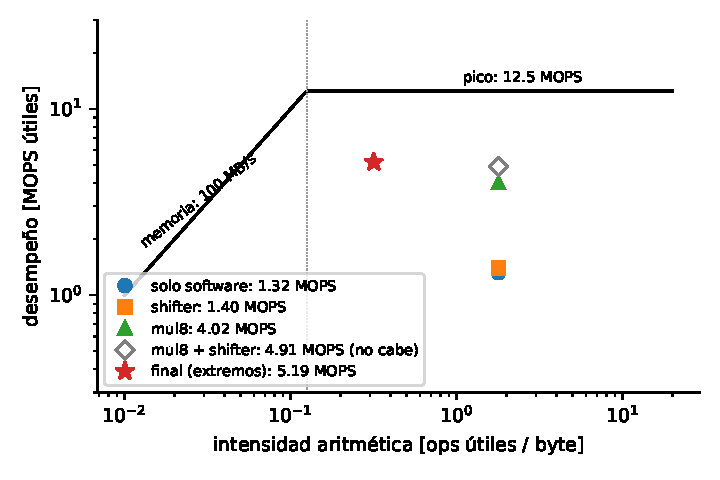
\includegraphics[width=\textwidth]{roofline.pdf}
\end{minipage}\hfill
\begin{minipage}{0.45\textwidth}
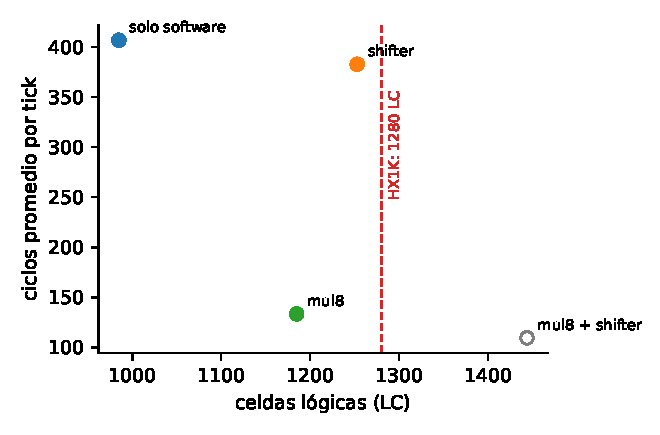
\includegraphics[width=\textwidth]{area_vs_ciclos.pdf}
\end{minipage}
\caption{Izquierda: roofline del Pochoco SoC \cite{roofline}, con las variantes del algoritmo anterior y el
algoritmo final (estrella). Derecha: celdas lógicas contra ciclos por tick del algoritmo anterior.
Fuente: elaboración propia.}
\label{fig:roofline}
\end{figure}

El roofline usa los techos vistos en clases. El de cómputo es una operación cada 2 ciclos,
12,5\,MOPS. El de memoria son 4 bytes por ciclo en el puerto de datos, 100\,MB/s. Se cruzan en
0,125 operaciones por byte. El kernel anterior mueve \BytesTick{} bytes por tick, contando los accesos a los
registros de la maestra, y su intensidad aritmética es \IntensidadOp{} operaciones por byte. Queda a
la derecha del cruce, limitado por cómputo y no por memoria.

La versión solo software corre a \MIPSSw{} MIPS, cerca del techo de 12,5. Pero cada multiplicación
cuesta unas 30 instrucciones, y solo logra \MopsSw{} millones de operaciones útiles por segundo. Con
\texttt{mul8} una multiplicación es una instrucción y sube a \MopsMul. Acelerar la memoria no habría
servido.

\subsection{Con el algoritmo final}

El estudio anterior buscó acelerar un kernel que multiplicaba. El algoritmo final no multiplica ni
desplaza: su tick toma \ExtCiclosProm{} ciclos, \ExtSpeedupMul{} veces menos que
el algoritmo anterior con \texttt{mul8} y \ExtSpeedupSw{} veces menos que el anterior solo por
software. Cambiar el algoritmo aceleró más que cualquier hardware que cabía en la FPGA.

Con ese kernel se revisaron otra vez las alternativas.
\begin{itemize}
\item \textbf{Multiplicador más rápido.} Un \texttt{mul8} de dos bits por ciclo (radix 4) bajaría su
latencia a la mitad. Con el algoritmo final hay cero multiplicaciones, así que no cambia nada. Con el
anterior, la multiplicación en hardware era cerca del 13\,\% de los ciclos y Amdahl da como máximo
$1/(1 - 0{,}13 \cdot 0{,}5) \approx 1{,}07$.
\item \textbf{Varios núcleos.} El SoC ocupa \LCSw{} de las 1280 celdas y el Espino es la mayor parte de
eso, así que un segundo núcleo no cabe en las \LCLibres{} que quedan. Además no hay nada que
repartir: llega un precio por tick y la decisión es una cadena de tres comparaciones que dependen una de
otra. La fracción paralelizable es cero y el speedup de Amdahl es 1.
\item \textbf{GPU (CUDA).} CUDA corre en tarjetas gráficas NVIDIA, no en la FPGA ni en el Espino. Sirve
para buscar parámetros fuera de línea. No hizo falta: \texttt{ref/competencia.py} simula 220 millones
de ticks (dos algoritmos, dos largos de ronda, \NVentanas{} ventanas) en unos 9 segundos en la CPU, con
numba.
\item \textbf{Decisión en hardware.} Las tres comparaciones podrían hacerse en el esclavo SPI, sin el
procesador. El tiempo de respuesta bajaría a cero, pero la plata sería la misma: la maestra igual lee
la decisión del tick anterior. Además el enunciado exige que la decisión se calcule en el Espino.
\end{itemize}

Lo que limita la ganancia ya no es el cómputo, sino el protocolo, que es igual para todos los grupos.
La decisión que se toma con el precio $p_n$ se ejecuta al precio $p_{n+1}$, y como $q \le 63$ entrar
y salir toma dos órdenes.

En el roofline el kernel final hace \ExtOpsTick{} operaciones útiles por tick y mueve
\ExtBytesTick{} bytes, una intensidad de 0,31 operaciones por byte. Sigue a la derecha del cruce
(0,125), limitado por cómputo. Logra \ExtMops{} MOPS útiles porque la mayoría de sus instrucciones
son de entrada y salida (leer NUEVO, escribir DECISION y los displays), no comparaciones.

También se evaluó \emph{recortar} el Espino a las instrucciones que usa el programa y poner varios
núcleos. El desglose de la síntesis da, en LUT: ALU 255, etapa ID 225, LSU 118, decoder 91 y fetch 62.
Un núcleo recortado (sin SUB, OR, XOR, SLT ni accesos de byte y media palabra) quedaría cerca de 400
LUT, pero cada núcleo sigue necesitando 4 BRAM para su banco de registros. Cuatro núcleos piden unas
1600 LUT y 16 BRAM más las 8 de la RAM: no caben en 1280 celdas y 16 BRAM. Y aunque cupieran, la plata
sería la misma y la latencia no bajaría, porque no hay trabajo que repartir. Lo que sí bajaría los
ciclos es mejorar el pipeline del núcleo (el CPI de \ExtCPI{} viene de la lectura sincrónica del banco
de registros), pero el programa ya usa el \ExtPctRtres\,\% de la ronda 3.

\subsection{Velocidad: el registro NUEVO y la lectura bloqueante}
\label{sec:velocidad}

En las prácticas con la maestra también se compararon tiempos de respuesta con ticks muy seguidos. La
maestra toma DECISION cuando baja CS. Entre el último bit de un precio y la bajada de CS siguiente
pasan 1\,$\mu$s más lo que sobre del período; con transacciones pegadas eso son unos 25 ciclos, menos
tres de sincronización. Con el programa anterior el peor caso precio $\to$ DECISION era 34 ciclos
(1,36\,$\mu$s), justo en los ticks en que la decisión cambia, porque actualizaba el piso y el techo antes
de escribir. Se hicieron tres cambios, midiendo cada uno en el testbench del curso.

\begin{enumerate}
\item \textbf{Software.} Cuando la decisión cambia, se escribe DECISION primero y el estado después.
\item \textbf{Esclavo SPI.} Un registro de solo lectura, NUEVO (offset \texttt{0x0C}), que entrega
$\{\text{precio nuevo}, 0, \text{precio}\}$; leerlo baja el aviso igual que leer PRICE. La espera queda en
\texttt{lw} y \texttt{bgez} en vez de \texttt{lw}, \texttt{andi}, \texttt{beqz} y la lectura de PRICE.
Peor caso: 16 ciclos.
\item \textbf{Núcleo: lectura bloqueante.} El esclavo SPI avisa (\texttt{wait\_o}) cuando se lee NUEVO
sin precio nuevo, y la unidad de carga del Espino no termina el \texttt{lw} mientras ese aviso esté
activo: repite la petición cada ciclo con el pipeline detenido, igual que cuando espera un dato de
memoria. Son cinco líneas en \texttt{espino\_load\_store\_unit.v} y un cable en el SoC. La espera
del programa pasa a ser un solo \texttt{lw}, que termina el ciclo siguiente a que llega el precio, sin
la granularidad de 6 ciclos de la vuelta de espera.
\end{enumerate}

Con los tres cambios el peor caso bajó de 34 a 9 ciclos sin ancla, 3,8 veces menos. El ancla de la
versión D agrega instrucciones antes del primer extremo y lleva el peor caso a \TbExtPeor{} ciclos
(0,48\,$\mu$s), todavía 2,8 veces menos que antes y muy bajo el presupuesto de \Presupuesto{} ciclos.
Las decisiones y la plata son las mismas. El diseño ocupa 985 celdas (Cuadro de síntesis). Las pruebas de instrucciones
siguen pasando en las cuatro variantes del núcleo, y la lectura bloqueante solo actúa sobre NUEVO, así
que un programa que no lo lea se comporta igual que en el Espino original.

También se evaluó repartir el trabajo en varios núcleos o en un núcleo de varios hilos. No baja la
latencia, porque llega un precio por tick y la decisión son comparaciones que dependen una de otra;
un núcleo con hilos intercalados además ejecuta cada hilo a un cuarto de la velocidad.

\subsection{Variante final}

El diseño de la competencia es el Espino sin \texttt{mul8} ni shifter y con la lectura bloqueante,
con la RAM con \texttt{no\_rw\_check} y el registro NUEVO en el esclavo SPI. Ocupa \LCSw{} celdas
(\LCPctSw\,\%) y su frecuencia máxima es \FmaxSw\,MHz. Las otras variantes siguen en el repositorio
detrás de \texttt{-DESPINO\_MUL8} y \texttt{-DESPINO\_SHIFTER}. El Cuadro~\ref{tab:final} pone el algoritmo
final (versión D) junto al anterior sobre el mismo hardware, para que se vea qué logró cada uno.

\begin{table}[H]
\centering\small
\caption{Algoritmo final (versión D) y algoritmo anterior sobre el mismo SoC, la variante final. LC son celdas
lógicas y BRAM bloques de 4\,kbit. El hardware es el mismo en las dos filas; solo cambia el programa.}
\label{tab:final}
\footnotesize\setlength{\tabcolsep}{3.5pt}
\begin{tabular}{lrrrrrrrrr}
\toprule
Algoritmo & LC & LUT4 & FF & BRAM & $f_\text{máx}$ [MHz] & Ciclos prom. & Ciclos peor & CPI & Mops útiles/s \\
\midrule
extremos (D) & \LCSw & 897 & 210 & 12 & \FmaxSw & \ExtCiclosProm & \ExtCiclosPeor & \ExtCPI & \ExtMops \\
tendencia (anterior) & \LCSw & 897 & 210 & 12 & \FmaxSw & \CiclosPromSw & \CiclosPeorSw & \CPISw & \MopsSw \\
\bottomrule
\end{tabular}
\fuente{Elaboración propia con \texttt{ref/sintesis.py} y \texttt{ref/verificar.py}; LUT4, FF y BRAM de \texttt{resultados/sintesis.csv}.}
\end{table}

Se eligió así porque el programa no usa \texttt{mul8} ni shifts, así que ese hardware solo gastaría
área, y porque es lo que se compila sin opciones, que es como corre el testbench del curso. Ni la
variante más rápida ni la que más acelera aporta algo con este algoritmo: la que mejor balancea LUTs,
ciclos y calidad de predicción es la más simple.

%=============================================================================
\section{Prueba en la placa y competencia}

\subsection{Prueba en la placa sin la maestra}

La simulación no ve todos los problemas. En el Proyecto 2 el SoC funcionaba en todas las simulaciones
y fallaba en la placa porque las BRAM no responden justo después de configurar la FPGA. Por eso se
probó el SoC en la Go Board sin la maestra del curso.

Se armó un bitstream aparte (\texttt{rtl/prueba\_placa}) con una maestra SPI dentro de la misma FPGA.
Le manda al SoC 1000 precios cada 0,1\,ms, el período de la ronda 3, con SCLK de 0,78\,MHz. Compara cada
byte leído con el que espera \texttt{trader.py} y muestra el resultado en los LEDs. Este bitstream no
se usa en la competencia, porque las reglas no permiten guardar series de precios en el diseño. Para
que la maestra cupiera junto al SoC se le sacó el contador de ciclos del Proyecto 2, que
\texttt{trade.s} no usa.

Los precios son dos tramos de la práctica nueva: 500 alrededor del máximo (donde el techo baja a 225) y
después 500 alrededor del mínimo (donde compra y el piso sube). Así la prueba pasa por todas las
ramas del programa. Primero se comprobó que la prueba detecta errores: en simulación pasa con la ROM
correcta y falla si se cambia un solo bit de un byte esperado.

El 17 de noviembre se grabó en la Go Board con el algoritmo de ese día. Los cuatro LEDs quedaron prendidos
fijos y los displays mostraron \texttt{A1}, el último precio de la prueba (161). Las 1001
transacciones dieron el byte que esperaba \texttt{trader.py}, al período de la ronda 3 y en el silicio
real.

La flash de la Go Board se programó sin cambiar el driver de Windows. Para eso se escribió un script
que hace lo mismo que \texttt{iceprog}, pero a través de la biblioteca del driver de FTDI que trae
Windows (\texttt{tools/goboard\_prog.py}).

\subsection{Pruebas con la maestra y versión grabada}

El 25 de noviembre se probaron con la maestra del curso las versiones G, F y D. La D fue la que mejor
se comportó, por decisión del grupo, y la placa quedó con ella (\texttt{grabar.ps1 -Version D}, con
verificación del grabado correcta). El bitstream final no se sube al repositorio (\texttt{.gitignore} excluye los \texttt{.bin}); se genera
con \texttt{make bin}. La competencia en vivo se corre con esa versión en las tres rondas.

%=============================================================================
\section{Conclusiones}

\begin{itemize}
\item La serie de práctica nueva cambió el algoritmo. Se reconstruyó exacta desde precios reales de Meta, y
eso mostró que cada serie de la competencia tiene su mínimo en 100 y su máximo en 255. Comprar en 100
y vender en 255 aprovecha esa propiedad. En \NVentanas{} ventanas posibles de las cinco empresas el
agente multiplica la plata por \ExtGeo{} en media geométrica, contra \CymGeo{} de comprar y mantener,
y pierde en el \ExtPierde\,\% de las ventanas, contra el \CymPierde\,\%. En la práctica termina con
\$\MetaW{} contra \$\MetaCym.

\item El programa no lleva contabilidad. Manda comprar 63 o vender 63 y deja que la maestra recorte la
orden. Así repetir una orden nunca hace daño, y el programa cabe en \ExtPalabras{} palabras sin multiplicar,
desplazar ni usar la RAM de datos.

\item El programa en assembly toma la misma decisión que Python en cada tick, salvo en los dos primeros, que llegan durante el reset de encendido. Se comprobó en un simulador
de instrucciones sobre \ExtNTicks{} ticks, en el RTL con el testbench del curso y en la placa. Un tick toma
\ExtCiclosProm{} ciclos en promedio y \ExtCiclosPeor{} en el peor caso, el \ExtPctRtres\,\% del tiempo de la
ronda 3.

\item En el estudio de co-diseño, hecho con el algoritmo anterior, la multiplicación por software era el
\FracMul\,\% de los ciclos y una instrucción propia y secuencial la redujo a pocos ciclos, con poca
área y sin perder frecuencia. El shifter aceleró menos y costó más. Las dos juntas no caben en la HX1K
y el PLL no existe en su encapsulado. Antes de agregar hardware hubo que liberar área: un atributo en
la memoria sacó unas 200 celdas que Yosys agregaba para un caso que el SoC nunca usa. La única mejora de
hardware que usa el programa final es el registro NUEVO con la lectura bloqueante, que baja el peor caso
precio $\to$ DECISION de 34 a 12 ciclos.

\item La mayor mejora no vino del hardware. Un algoritmo mejor hizo el tick \ExtSpeedupMul{} veces más corto
que la mejor variante de hardware del algoritmo anterior, y permitió volver al Espino sin instrucciones
nuevas. Es la ley de Amdahl vista desde el otro lado: acelerar una parte que el algoritmo ya no necesita
no sirve.

\item Limitaciones: la regla depende de que las series de la competencia estén normalizadas entre 100 y
255 como la práctica; con rondas cortas (2000 ticks) el agente casi no opera y pierde en el
\ExtCortaPierde\,\% de las ventanas; el 225, el 122 y el ancla de 29 se ajustaron con datos de 2022 a
2024; y el estudio de co-diseño se hizo con el algoritmo anterior, no con el final. La comparación
tick a tick contra el RTL de la serie de práctica completa coincide salvo en los dos primeros ticks, que llegan
durante el reset de encendido del SoC.
\end{itemize}

%=============================================================================
\begin{thebibliography}{9}
\bibitem{enunciado} J. Gómez Mir. \emph{Proyecto 4: Pochoco Trader. Co-diseño hardware/software sobre
Espino Core}, Arquitectura de Computadores, Universidad de los Andes, 2026-2.
\bibitem{pochoco} N. Villegas. \emph{Pochoco SoC} (repositorio base del curso).
\url{https://github.com/nic0villegasc/pochoco_soc}
\bibitem{repo} Grupo 2. \emph{Proyecto 4 Arquitectura de Computadores}.
\url{https://github.com/F-Izcue-223/Proyecto-4-Arquitectura-de-Computadores}
\bibitem{riscv} RISC-V International. \emph{The RISC-V Instruction Set Manual, Volume I: Unprivileged
ISA} (RV32E y espacio custom-0). \url{https://docs.riscv.org/reference/isa/v20260120/unpriv/rv32.html}
\bibitem{hp} J. Hennessy y D. Patterson. \emph{Computer Architecture: A Quantitative Approach}, 6.ª ed.
Morgan Kaufmann, 2017 (ley de Amdahl).
\bibitem{roofline} S. Williams, A. Waterman y D. Patterson. ``Roofline: an insightful visual performance
model for multicore architectures''. \emph{Communications of the ACM}, 52(4), 2009.
\bibitem{lattice} Lattice Semiconductor. \emph{iCE40 LP/HX Family Data Sheet} (PLL por encapsulado).
\bibitem{naval} E. Jorgenson. \emph{El almanaque de Naval Ravikant}. Colección Baelo, 2021.
\bibitem{goboard} Nandland. \emph{The Go Board}. \url{https://nandland.com/the-go-board/}
\bibitem{yosys} YosysHQ. \emph{Yosys Open SYnthesis Suite documentation}.
\url{https://yosyshq.readthedocs.io/en/latest/}
\end{thebibliography}

%=============================================================================
\clearpage
\section*{Declaración de Uso de Herramientas de Inteligencia Artificial}
\addcontentsline{toc}{section}{Declaración de Uso de Herramientas de Inteligencia Artificial}

% REVISAR POR EL GRUPO antes de entregar: la declaracion es del grupo (fechas, herramientas y alcance).
\subsection*{1. Identificación de la actividad}
\begin{itemize}
\item \textbf{Curso:} Arquitectura de Computadores
\item \textbf{Código del curso:} 433
\item \textbf{Nombre de la actividad:} Proyecto N°4
\item \textbf{Fecha de entrega:} \FechaEntrega
\item \textbf{Nombre(s) de(los) estudiante(s):} Josefa Alcaíno Lira, Felipe Izcúe Ferrer, Martín Norton Haigis
\end{itemize}

\subsection*{2. Declaración sobre uso de IA}
$\square$ No se utilizaron herramientas de inteligencia artificial en ninguna etapa del desarrollo de esta
actividad.\\
$\boxtimes$ Sí se utilizaron herramientas de inteligencia artificial, según se detalla en la sección 3 de este
documento.

\clearpage
\subsection*{3. Descripción de uso de IA}
\vspace{4pt}
\renewcommand{\arraystretch}{1.25}
\noindent\begin{tabular}{|p{4.7cm}|p{11.3cm}|}
\hline
\textbf{Herramienta empleada} & Claude (Anthropic): Opus 5.5 y Sonnet 5.5 \\ \hline
\textbf{Fechas de uso} & Entre el 5 y el 27 de noviembre de 2026 \\ \hline
\textbf{Estudiantes} & Josefa Alcaíno Lira, Felipe Izcúe Ferrer y Martín Norton Haigis \\ \hline
\textbf{Propósito del uso} & Diseño y validación del algoritmo de inversión y del optimizador (Python),
escritura de \texttt{trade.s} y de las variantes de co-diseño, modificaciones al RTL (multiplicador
\texttt{mul8}, shifter y lectura bloqueante del esclavo SPI), testbenches y scripts de simulación,
síntesis y grabado de la placa. Análisis de los resultados, elaboración de las tablas y figuras, y apoyo
en la redacción del informe en LaTeX, del README, de la guía de la defensa y en la organización y
subida del repositorio. \\ \hline
\textbf{Descripción de integración} & Claude se usó de forma iterativa: el grupo planteaba el problema, Claude
escribía el código, el script o el texto, y el grupo lo revisaba, lo ejecutaba y pedía correcciones. El
grupo ejecutó las pruebas con la maestra y en la placa, y Claude leyó los resultados para armar las
tablas y los gráficos y redactó el informe. Todo el contenido fue revisado por el grupo, que es
responsable de poder explicarlo y defenderlo. \\ \hline
\end{tabular}

\end{document}
